%\documentclass[reviewcopy]{elsart}
\documentclass{elsart}
% Use the option doublespacing or reviewcopy to obtain double line spacing
% \documentclass[doublespacing]{elsart}
\usepackage{natbib}
%\usepackage{endfloat}           % Float pics to the end
\usepackage{color}
\usepackage{url}
\usepackage{graphicx}
\usepackage{subfigure}
\usepackage{units}
\usepackage{amsmath}

\input{../cimis_acronyms} % CIMIS Acronyms

\begin{document}
%
\begin{frontmatter}
  \title{Daily reference evapotranspiration for California using
    satellite imagery and weather station measurement interpolation}
%
\author[calspace]{Quinn~Hart\corauthref{cor}}
\corauth[cor]{Corresponding author.}
\ead{qjhart@ucdavis.edu}
\author[calspace]{Marcela~Brugnach\thanksref{marcela}}
\ead{mbrugnac@usf.uos.de}
\author[cimis]{Bekele~Temesgen}
\ead{temesgen@water.ca.gov}
\author[calspace]{Carlos~Rueda}
\ead{carueda@ucdavis.edu}
\author[calspace]{Susan~Ustin}
\ead{slustin@ucdavis.edu}
\author[cimis]{Kent~Frame}
\ead{kframe@water.ca.gov}

\address[calspace]{CalSpace, University of California, Davis, Davis, CA, USA }

%\address[marcela]{Institute of Environmental Systems Research \\
%University of Osnabrueck  \\
%Germany }
\thanks[marcela]{Currently: Institute of Environmental Systems
  Research, University of Osnabrueck, Germany }

\address[cimis]{California Irrigation Management Information System
  (CIMIS), California Department of Water Resources, Sacramento, CA,
  USA }

\begin{abstract}
  Spatially distributed \ac{ET0} is calculated to produce daily
  \ac{ET0} maps for the State of California at high spatial
  resolution, $(\unit[2]{km})^2$.  Hourly \acs{NOAA} \acs{GOES} visible
  channel imager data are used to modify modeled radiation estimates.
  These are combined with interpolated \acf{CIMIS} weather station
  meteorological data to satisfy the Penman-Monteith \ac{ET0}
  equation.  Data have been acquired and \ac{ET0} estimated daily from
  February 2003 through April 2006.
\end{abstract}

\begin{keyword}
% keywords here, in the form: keyword \sep keyword
  evapotranspiration \sep Penman-Monteith equation \sep satellite
  imaging \sep remote sensing
% PACS codes here, in the form: \PACS code \sep code
% http://www.aip.org/pacs
\PACS 92.40.Zg \sep 92.40.Je \sep 42.68.Wt
\end{keyword}
\end{frontmatter}                                

% This format puts a special copyright style on the first page
%\thispagestyle{plain}


\section{Average \ac{ET0} values}

Although the main goal of producing daily \ac{ET0} maps is to provide
support for short term irrigation strategies, examination of long term
averages can provide insight into major \ac{ET} regimes in California,
and provide validation of the model when compared to similar maps.
Approximately 3 years of data for each month were combined to provide
12 monthly averages of \ac{ET0} throughout California.  A \ac{PCA}
transformation~\citep{richards86remot-sensin} was applied to these 12
values, and the top three components were used in an unsupervised
classification of California's \ac{ET0} zones.
Figure~\ref{fig:pca_graph} shows the contributions of the monthly
\ac{ET0} values to each \ac{PCA} vector.  These components can be
roughly identified as picking out the total yearly amount of \ac{ET0}
for a pixel and the spring and summer contributions to the \ac{ET0}.

\begin{figure}
  \centering
  \begin{picture}(0,0)%
\includegraphics{monthly/pca_fig.pdf}%
\end{picture}%
\setlength{\unitlength}{3947sp}%
%
\begingroup\makeatletter\ifx\SetFigFont\undefined%
\gdef\SetFigFont#1#2#3#4#5{%
  \reset@font\fontsize{#1}{#2pt}%
  \fontfamily{#3}\fontseries{#4}\fontshape{#5}%
  \selectfont}%
\fi\endgroup%
\begin{picture}(3747,2257)(1271,-3950)
\put(1763,-3773){\makebox(0,0)[rb]{\smash{{\SetFigFont{10}{12.0}{\familydefault}{\mddefault}{\updefault}-0.6}}}}
\put(1763,-3496){\makebox(0,0)[rb]{\smash{{\SetFigFont{10}{12.0}{\familydefault}{\mddefault}{\updefault}-0.4}}}}
\put(1763,-3219){\makebox(0,0)[rb]{\smash{{\SetFigFont{10}{12.0}{\familydefault}{\mddefault}{\updefault}-0.2}}}}
\put(1763,-2942){\makebox(0,0)[rb]{\smash{{\SetFigFont{10}{12.0}{\familydefault}{\mddefault}{\updefault} 0}}}}
\put(1763,-2664){\makebox(0,0)[rb]{\smash{{\SetFigFont{10}{12.0}{\familydefault}{\mddefault}{\updefault} 0.2}}}}
\put(1763,-2387){\makebox(0,0)[rb]{\smash{{\SetFigFont{10}{12.0}{\familydefault}{\mddefault}{\updefault} 0.4}}}}
\put(1763,-2110){\makebox(0,0)[rb]{\smash{{\SetFigFont{10}{12.0}{\familydefault}{\mddefault}{\updefault} 0.6}}}}
\put(1763,-1833){\makebox(0,0)[rb]{\smash{{\SetFigFont{10}{12.0}{\familydefault}{\mddefault}{\updefault} 0.8}}}}
\put(1838,-3898){\makebox(0,0)[b]{\smash{{\SetFigFont{10}{12.0}{\familydefault}{\mddefault}{\updefault}Jan}}}}
\put(2100,-3898){\makebox(0,0)[b]{\smash{{\SetFigFont{10}{12.0}{\familydefault}{\mddefault}{\updefault}Feb}}}}
\put(2345,-3898){\makebox(0,0)[b]{\smash{{\SetFigFont{10}{12.0}{\familydefault}{\mddefault}{\updefault}Mar}}}}
\put(2598,-3898){\makebox(0,0)[b]{\smash{{\SetFigFont{10}{12.0}{\familydefault}{\mddefault}{\updefault}Apr}}}}
\put(2852,-3898){\makebox(0,0)[b]{\smash{{\SetFigFont{10}{12.0}{\familydefault}{\mddefault}{\updefault}May}}}}
\put(3105,-3898){\makebox(0,0)[b]{\smash{{\SetFigFont{10}{12.0}{\familydefault}{\mddefault}{\updefault}Jun}}}}
\put(3359,-3898){\makebox(0,0)[b]{\smash{{\SetFigFont{10}{12.0}{\familydefault}{\mddefault}{\updefault}Jul}}}}
\put(3612,-3898){\makebox(0,0)[b]{\smash{{\SetFigFont{10}{12.0}{\familydefault}{\mddefault}{\updefault}Aug}}}}
\put(3874,-3898){\makebox(0,0)[b]{\smash{{\SetFigFont{10}{12.0}{\familydefault}{\mddefault}{\updefault}Sep}}}}
\put(4127,-3898){\makebox(0,0)[b]{\smash{{\SetFigFont{10}{12.0}{\familydefault}{\mddefault}{\updefault}Oct}}}}
\put(4381,-3898){\makebox(0,0)[b]{\smash{{\SetFigFont{10}{12.0}{\familydefault}{\mddefault}{\updefault}Nov}}}}
\put(4634,-3898){\makebox(0,0)[b]{\smash{{\SetFigFont{10}{12.0}{\familydefault}{\mddefault}{\updefault}Dec}}}}
\put(4888,-3898){\makebox(0,0)[b]{\smash{{\SetFigFont{10}{12.0}{\familydefault}{\mddefault}{\updefault}Jan}}}}
\put(1387,-2741){\rotatebox{90.0}{\makebox(0,0)[b]{\smash{{\SetFigFont{10}{12.0}{\familydefault}{\mddefault}{\updefault}Weight}}}}}
\put(4288,-1970){\makebox(0,0)[rb]{\smash{{\SetFigFont{10}{12.0}{\familydefault}{\mddefault}{\updefault}PC1: Yearly Total}}}}
\put(4288,-2095){\makebox(0,0)[rb]{\smash{{\SetFigFont{10}{12.0}{\familydefault}{\mddefault}{\updefault}PC2: Summer Values}}}}
\put(4288,-2220){\makebox(0,0)[rb]{\smash{{\SetFigFont{10}{12.0}{\familydefault}{\mddefault}{\updefault}PC3: Spring Values}}}}
\end{picture}%

  \caption{Three most important principle
    component vectors for monthly contribution to \ac{ET0}}
\label{fig:pca_graph}
\end{figure}

An unsupervised classification of 6 regions derived from these
\ac{PCA} vectors is shown in Figure~\ref{fig:et0-classes}.  These are
generally labeled with their prominent location within California.
Given these regions, summary information about expected \ac{ET0}
amounts through the year can be calculated.  These are shown in
Table~\ref{tab:et0-classes}, which describes the average \ac{ET0} for
each region and month.

\begin{figure}
  \centering
  \includegraphics[width=1\textwidth]{monthly/classes.png}  
  \caption{Unsupervised classification \ac{ET0} regions based on three
    years of data.}
  \label{fig:et0-classes}
\end{figure}

\begin{table}
  \centering
  \caption{Average \ac{ET0} values for different California regions}
  \begin{tabular}{c|c|c|c|c|c|c|c}
& South & South & Northern & Mojave & Coast & High & Central \\
Month & Coast & Valley & Mountains & Desert & Range & Sierra & Valley \\
\hline \hline
Jan & 1.68 & 0.88 & 0.73 & 2.01 & 1.47 & 0.75 & 0.88 \\
Feb & 2.13 & 1.68 & 1.46 & 2.69 & 2.11 & 1.47 & 1.69 \\
Mar & 3.01 & 2.93 & 2.54 & 4.38 & 3.35 & 2.61 & 2.88 \\
Apr & 3.60 & 3.85 & 2.93 & 5.57 & 4.15 & 2.99 & 3.61 \\
May & 4.40 & 5.28 & 4.23 & 7.22 & 5.49 & 4.26 & 4.90 \\
Jun & 4.52 & 6.47 & 5.78 & 8.25 & 6.40 & 5.65 & 6.06 \\
Jul & 5.33 & 6.87 & 6.50 & 8.21 & 6.90 & 6.51 & 6.48 \\
Aug & 4.94 & 6.05 & 5.47 & 7.20 & 6.22 & 5.55 & 5.73 \\
Sep & 4.10 & 4.78 & 4.20 & 6.20 & 5.09 & 4.29 & 4.65 \\
Oct & 2.62 & 2.76 & 2.35 & 3.86 & 3.13 & 2.42 & 2.77 \\
Nov & 1.98 & 1.36 & 1.04 & 2.24 & 1.86 & 1.08 & 1.33 \\
Dec & 1.54 & 0.88 & 0.68 & 1.80 & 1.40 & 0.70 & 0.86 \\    
  \end{tabular}
  \label{tab:et0-classes}
\end{table}

The Department of Water Resources and UC Davis, have previously
developed a map of \ac{ET0} zones in
California~\citep{cimis99calif-refer}, shown in Figure~\ref{fig:et0}.
This map was the result of experts delineating regions in California,
based on long term weather station data.  Comparison of this map to
that of Figure~\ref{fig:et0-classes} show good agreement, and provide
a qualitative validation of the \ac{GOES} and \ac{CIMIS} derived map
products.

\begin{figure}[htbp]
  \centering
  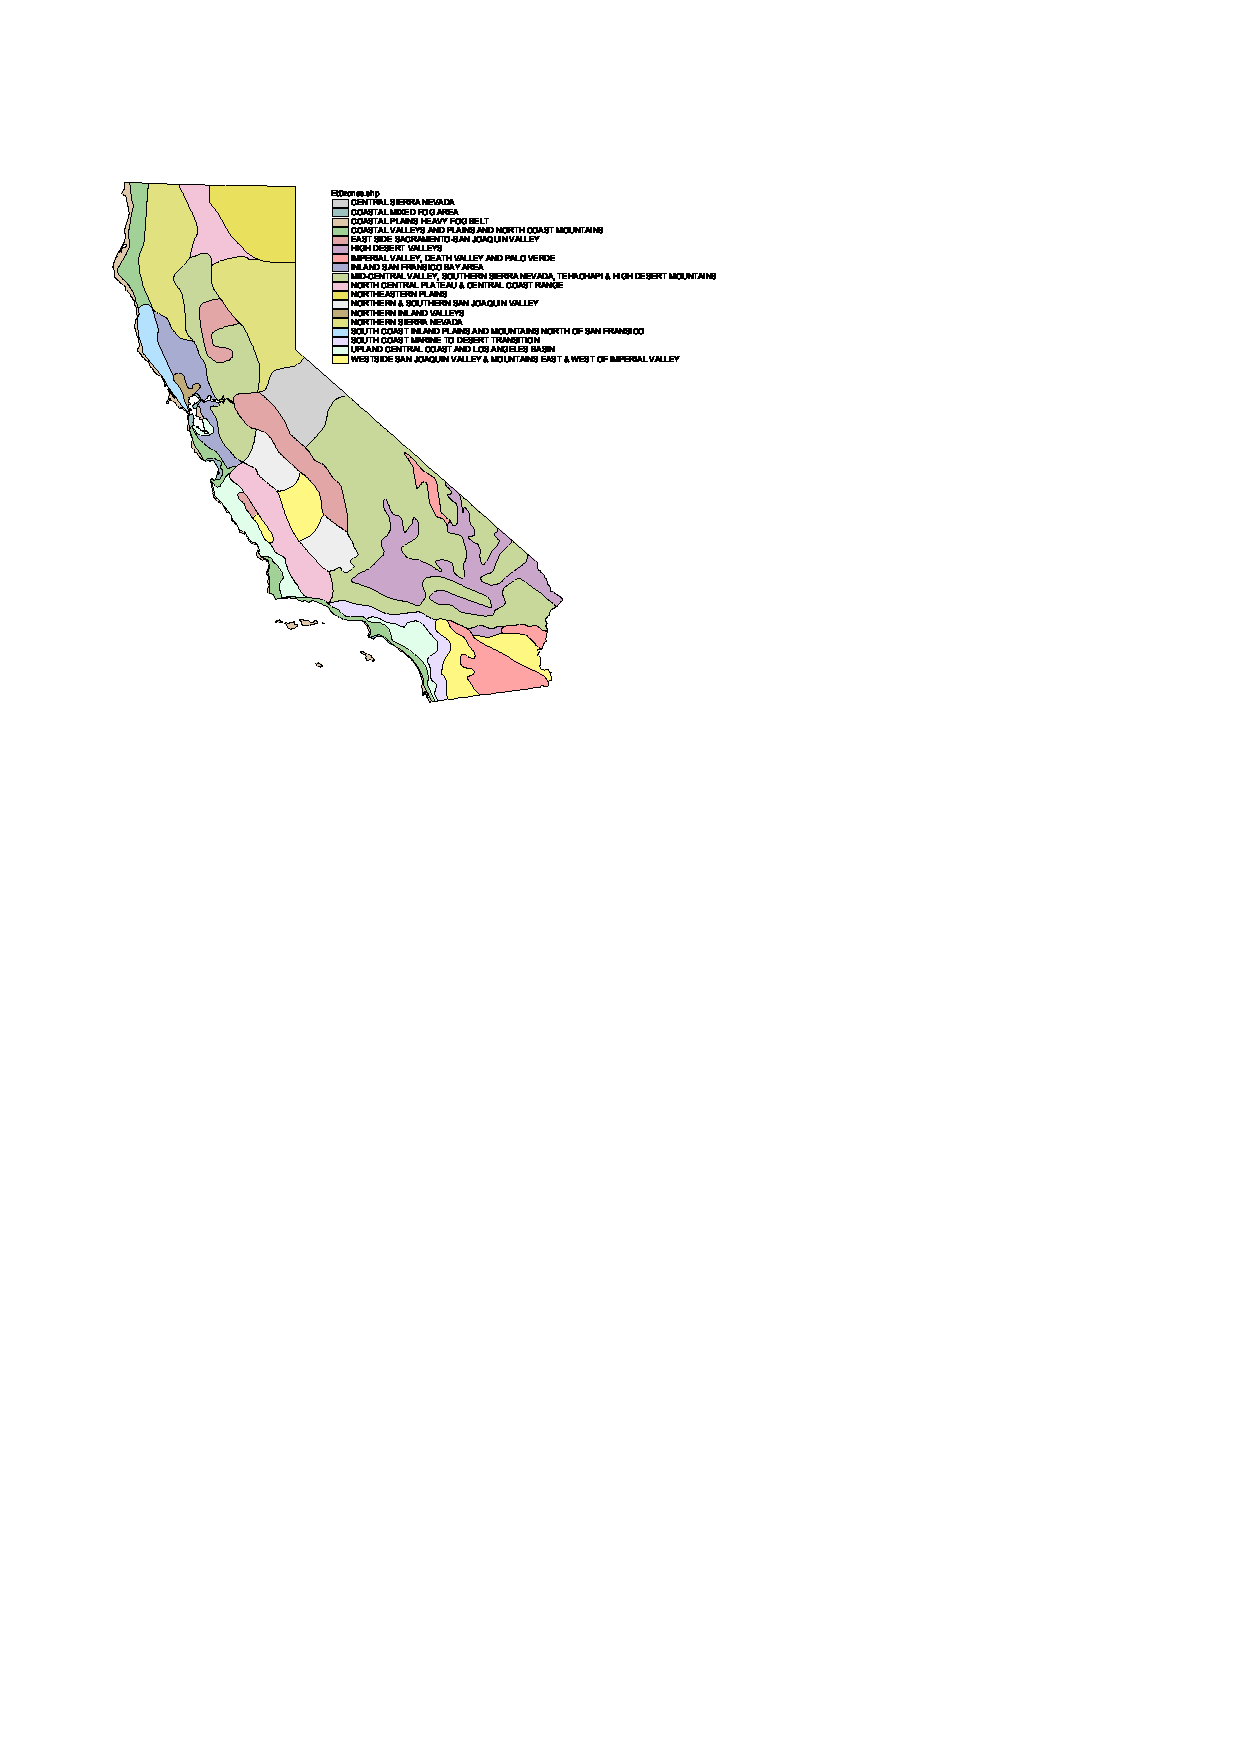
\includegraphics[width=1\textwidth]{etomap_simple.pdf}
  \caption{%
    Map of different \ac{ET0} zones for California.  18 separate
    zones, derived from monthly \ac{ET0} averages, delineate different
    regions and influences in California. }
  \label{fig:et0}
%\vspace*{12pt}\hrule
\end{figure}

\end{document}


% LocalWords:  evapotranspiration albedo irradiance imager snowpack snowmelt streamflow CIMIS FAO
% LocalWords:  stomata micrometeorological Monteith emissitivity Linke isolines
% LocalWords:  psychrometric Heliosat turbidity sigmoidal longwave DayMet